% !TEX root = ../main.tex
\subsection{The Galaxy Sample}
The galaxies selected analysed in this paper are the 198 galaxies from \comment{Lingard et al, in prep.}. We combine classifications of galaxies which were repeated in the \textit{validation subset} with the original classifications. Clustering of drawn spiral arms and cleaning of points was then performed as detailed in \comment{Lingard et al, in prep.}. We remove any galaxies for which no arms were identified. This results in a hierarchiacal data structure of 109 galaxies, 250 spiral arms and 307,861 points.

Spiral arm points are deprojected to a face-on orientation using the position angle \textsc{PETRO\_PHI90} and axis ratio \textsc{PETRO\_BA90} keywords from the NASA-Sloan Atlas \comment{citation}. We scale the radii to have unit variance (which does not impact log spiral pitch angle due to its scale invariance).

\comment{Should I elaborate more on the sample?}

\subsection{Bayesian modelling of spiral arms in \textit{Galaxy Builder}}

We model a spiral arm as a logarithmic spiral, described by

\begin{equation}
r_\mathrm{arm} = \exp\left[\theta_\mathrm{arm}\tan\phi_\mathrm{arm} + c_\mathrm{arm}\right].
\end{equation}

Assume the pitch angle of a galaxy's spiral arms are drawn from a Normal distribution, truncated between 0 and 90 degrees, centred on some value we will call the galaxy's pitch angle, $\phi_\mathrm{gal}$. This dispersion in arm pitch angle has some measure of spread, $\sigma_\mathrm{gal}$, which we will assume is the same in galaxies:

\begin{equation}
\phi_\mathrm{arm} \sim \mathrm{TruncatedNormal}(\phi_\mathrm{gal}, \sigma_\mathrm{gal}, \mathrm{min}=0, \mathrm{max}=90).
\end{equation}

We choose hyperpriors on $\phi_\mathrm{gal}$ and $\sigma_\mathrm{gal}$ of

\begin{align}
  \phi_\mathrm{gal} &\sim \mathrm{Uniform}(\mathrm{min}=0, \mathrm{max}=90),\\
  \sigma_\mathrm{gal} &\sim \mathrm{InverseGamma}(\alpha=2,\,\beta=20).
\end{align}

We also have the offset parameter $c$, and a measure of radial uncertainty $\sigma_r$:

\begin{align}
  c_\mathrm{arm} &\sim \mathrm{Cauchy}(\alpha=0,\,\beta=10),\\
  \sigma_r &\sim \mathrm{HalfCauchy}(\beta=0.2).
\end{align}

\begin{figure}
  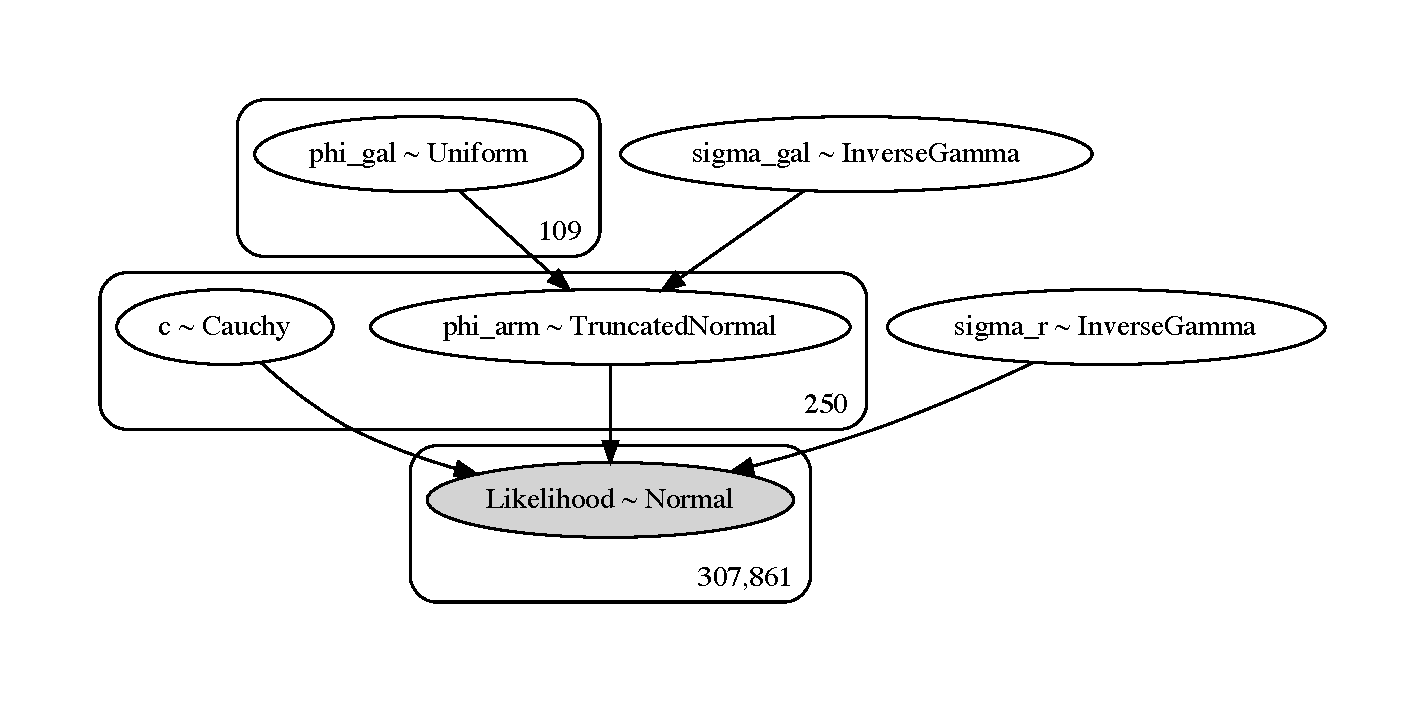
\includegraphics[width=8cm]{plots/plots_n109d1000t500/model.pdf}
  \caption{The model used for galaxy pitch angle measurement for the sample.}
  \label{fig:pymc3-model}
\end{figure}

To perform inference, we make use of the No-U-Turn-Sampler (NUTS, \citealt{2011arXiv1111.4246H}), implemented in PYMC3\footnote{\url{https://docs.pymc.io/}}, an open source probabilistic programming framework written in python \citep{pymc3_paper}.
